\documentclass[12pt]{article}
\usepackage[a4paper, total={6in, 10in}]{geometry}

\usepackage{graphicx}
\usepackage{abstract}
\usepackage{hyperref}
\usepackage{listings}
\usepackage{indentfirst}
\usepackage{amssymb}
\usepackage{titling}
\usepackage{mwe}
\usepackage{fancyhdr}
 
\graphicspath{ {./images/} }
\renewcommand{\abstractname}{\small{\begin{center}Timestamps\end{center}\vspace{-4ex}}}

\setlength{\parskip}{3mm}   % Add space between paragraphs.
\setlength{\parindent}{0.5in}
\setlength{\droptitle}{-35pt}
\linespread{1.2}

\fancypagestyle{plain}{
    \vspace{3ex}
    \fancyhead[L]{October 10th, 2020}
    \renewcommand{\headrulewidth}{0.5pt}
}

\pretitle{\begin{center} \LARGE \textbf}
\posttitle{\end{center} \vspace{-3ex}}
\preauthor{\begin{center} \large}
\postauthor{\end{center} \vspace{-3ex}}
\predate{\begin{center} \small \emph}
\postdate{\end{center} \vspace{-3ex}}

\title{Chapter 4 \& 5 Summary}
\author{Chris Nutter\thanks{Dedicated to @QuesoGrande a.k.a. Jared D.}}
\date{CPSC 362}

% --> Here we go, satellite radio, y'all get hit with a...

\begin{document}
\maketitle

\begin{center} \vspace{-4ex}|\vspace{-3ex} \end{center}

\noindent\abstractname
\begin{center}
    \normalsize\textbf{10/08/2020 - 01:58:55 PM}\\
    Figures of each model are at the end of the document.
\end{center}
\normalsize

\tableofcontents    
\vspace{4ex}

% --> First Chapter

\section{Chapter 4}
\indent 
\emph{Prescriptive Process Model} is about constructing the order of software development where each task is set in order with specified guidelines. 
\emph{The Waterfall Model} sets a sequential method to development with no traversal to earlier or later stages (similar to a waterfall that goes straight down and not back up again). 
\emph{Incremental Process Model} relies on both linear and parallel processing directions to be applied; linear being the sequence of events while jumping around through increments \#n. 
\emph{Evolutionary Process Model} is very iterative which constantly improves upon over time before reaching the final product. It keeps adding to the itself which makes the project bigger and closer to the final product. 
\emph{Prototyping} is an important step to test your project and practically mandatory for releasing a product. Prototyping is often sent out to testers as a way of getting accurate reception of a product without in-house teams to influence judgement. For example a team creates a math game for 1st graders. The team will give the product to 1st graders to see how they like the product.
\emph{The Spiral Model} is a combination of prototyping with the Waterfall Model method which is very useful for fast development of versions for teams that are stuck in a time constraint.
\emph{Concurrent Model or sometimes concurrent engineering} is the repetitive nature of any process model mentioned.
\emph{Specialized Process Models} take one or more attributes of other models into one model.
\emph{Component-Based Development} is a special model that has many Spiral Model features with pre-packaged software components. There are 5 stages to the component-based development model.
    \begin{enumerate}
        \item Available component-based products are researched and evaluated for 
        the application domain in question.  
        \item Component integration issues are considered.  
        \item A software architecture is designed to accommodate the components.  
        \item Components are integrated into the architecture.
        \item Comprehensive testing is conducted to ensure proper functionality.  
    \end{enumerate}
\emph{Aspect-Oriented Software Development} is the process and methodological way of defining, specifying, designing, and constructing \emph{aspects}.
\emph{Aspects} are ways of sub-routing and localizing the expression of crosscutting concerns.
\emph{Concerns} are the required parameters of a customer.
Putting it all together, \emph{crosscutting concerns} are concerns that are cut across various functions, features, and information bases.
\emph{Unified Process} recognises importance with customer communication towards the end goal.
    \begin{enumerate}
        \item \emph{Inception} or communication and planning
        \item \emph{Elaboration} or planning and modelling
        \item \emph{Construction}
        \item \emph{Transition} or construction to deployment
        \item \emph{Production} or software implement
    \end{enumerate}
\emph{Personal Software Process} is similar to unified process but for personal development.
    \begin{enumerate}
        \item \emph{Planning} requires isolation of requirements
        \item \emph{High-level design} requires component construction and design
        \item \emph{High-level design review} requires verification methods to find error
        \item \emph{Development} is for design refining.
        \item \emph{Postmortem} is the collected measure of each stage to analyse effectiveness.
    \end{enumerate}
\emph{Team Software Process} is similar to PSP but requires a further team-based curriculum to tackle. Various team building suggestions include moral boosting seminars, planning goals accordingly, accelerate process by coaching, providing guidance in a respectable manner, and facilitate university teaching.

\section{Chapter 5}
\indent 
\emph{Agility} is very important and widely spread across software engineering. Ivar Jacobson says "Everyone is agile. An agile team is a nimble team able to appropriately respond to changes." Agility involves the philosophy of team structures and team attitudes being used among the members including technicians, programmers, design, everyone. Agility should be applied to any software process but it is essential to understand how agility is adapted to various different processes' tasks. Agile development processes lowers the development cost compared to conventional software processes and also increases development schedule processes.\\ 
\indent 
Agile software process is mentioned as the manner of addressing a number of assumption about the majority of software projects. Agility principles are important for understanding and working towards and agile software process.
    \begin{enumerate}
        \item Our highest priority is to satisfy the customer through early and continuous delivery of valuable software.
        \item Welcome changing requirements, even late in development. Agile processes harness change for the customer's competitive advantage.  
        \item Deliver working software frequently, from a couple of weeks to a couple of months, with a preference to the shorter timescale.  
        \item Business people and developers must work together daily throughout the project. 
        \item Build projects around motivated individuals. Give them the environment and support they need, and trust them to get the job done.  
        \item The most efficient and effective method of conveying information to and within a development team is face-to-face conversation.
        \item Working software is the primary measure of progress.
        \item Agile processes promote sustainable development. The sponsors, developers, and users should be able to maintain a constant pace indefinitely.  
        \item Continuous attention to technical excellence and good design enhances agility.  
        \item Simplicity—the art of maximizing the amount of work not done—is essential.  
        \item The best architectures, requirements, and designs emerge from self organizing teams.  
        \item At regular intervals, the team reflects on how to become more effective, then tunes and adjusts its behavior accordingly.  
    \end{enumerate}
The agile software process is very important to a proper work ethic that is fast and efficient for all parties.\\
\indent
\emph{The XP Process} is the object-oriented approach as a preferred development paradigm. It is labeled as the Extreme Programming for a reason. Planning the process requires listening to the people and technical members. Design which requires rigorous principles to follow by which are \textbf{keeping it simple}. Coding which is expanitory which is preliminary design implemented over time. It's not immediately ported over and needs tweaking and subtle improvements/adjustments over time. Lastly, testing which is crucial to a healthy design. Many errors will be made so adjusting and finding acceptable levels is appropriate at this step.
\emph{Scrum} is a development method that are consistent with the agile "manifesto" and are framed into 5 basic activities.
    \begin{enumerate}
        \item Requirements
        \item Analysis
        \item Design
        \item Evolution
        \item Delivery.
    \end{enumerate}
Each framework allocates different important step to an appropriate manifesto.
\emph{Agile Unified Process} adopts a "serial in the large" and "iterative in the small" philosophy. Adopting the previous iteration's activities and working upon them in this one is essential and allows for updated output.\\
\indent
A proper agile philosophy permits a proper engineering ethic for everyone. These tools help facilitate a proper agile working habit for all members which is important for succeeding in the engineering field. Ever since the dawn of humans, we have been all been collaborating using different strengths to solve the same problems.

\newpage

\section{Images}

    \begin{figure}[hbtp]
        \centering
        \fbox{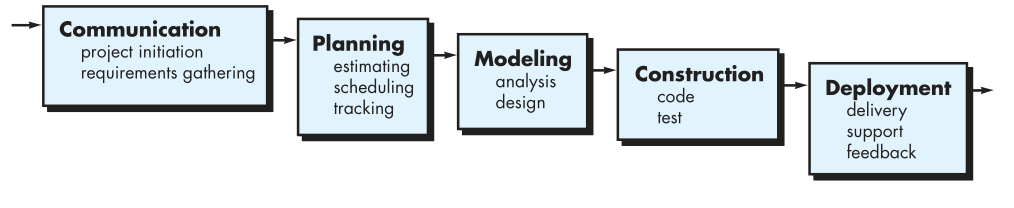
\includegraphics[width=13.8cm]{waterfall.png}}
        \caption{Waterfall Model}
    \end{figure}
    \begin{figure}[hbtp]
        \centering
        \fbox{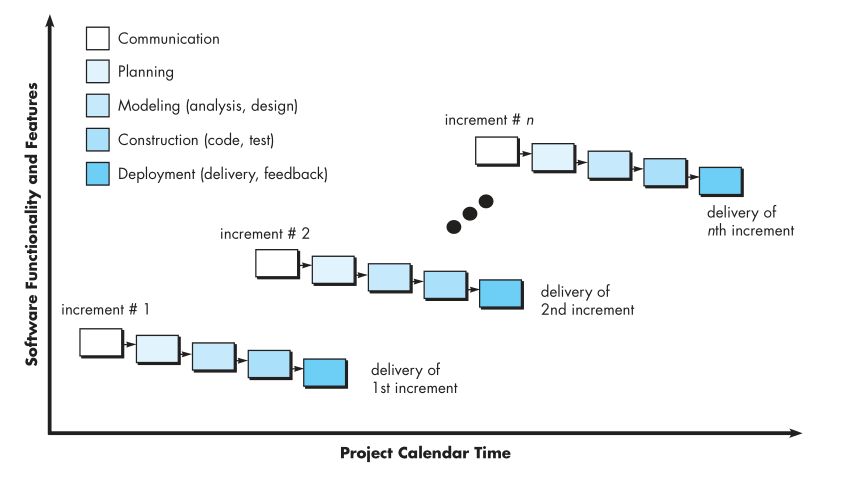
\includegraphics[width=13.8cm]{inc.png}}
        \caption{Incremental Model}
    \end{figure}
    \begin{figure}[hbtp]
        \centering
        \fbox{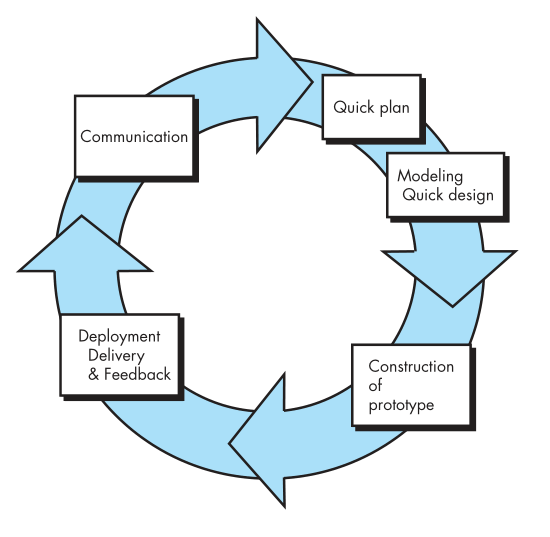
\includegraphics[width=6.8cm]{proto.png}}
        \caption{Prototyping}
    \end{figure}
    \begin{figure}[hbtp]
        \centering
        \fbox{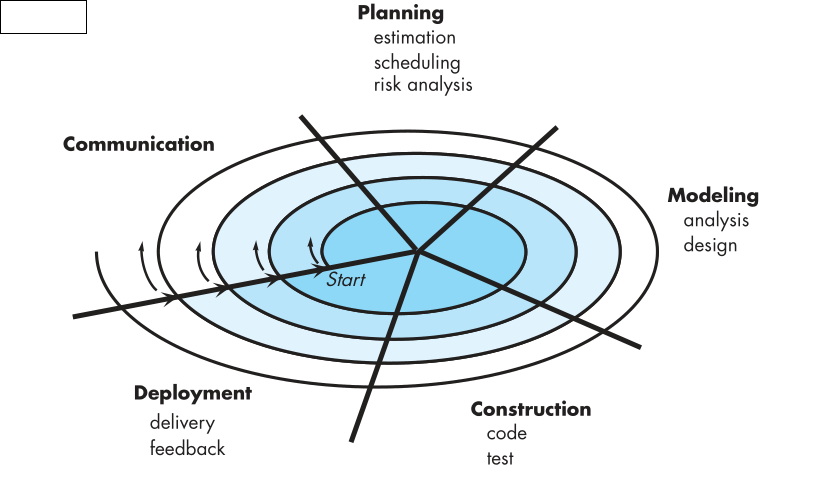
\includegraphics[width=13.8cm]{spiral.png}}
        \caption{Spiral Model}
    \end{figure}
    \begin{figure}[hbtp]
        \centering
        \fbox{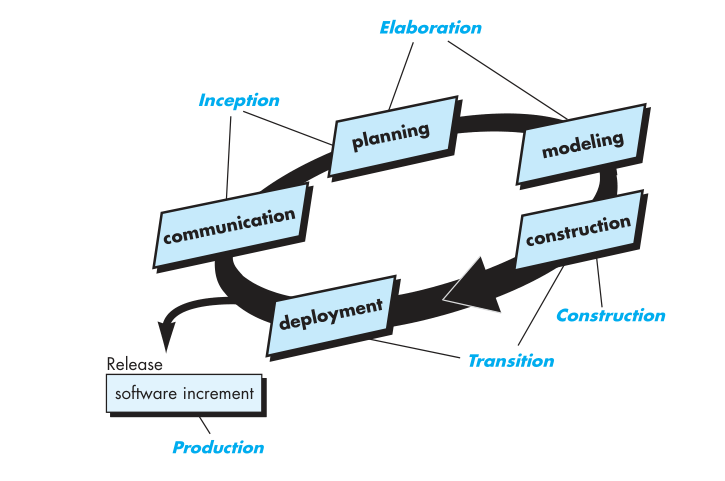
\includegraphics[width=13.8cm]{unified.png}}
        \caption{Unified Model}
    \end{figure}

\end{document}
